\chapter{Értékelés}

\section{Mérések}

\subsection{Hálózati kommunikáció}
A hálózati kommunikáció esetében tesztelve lett Wireshark segítségével a hálózat felépítése és meghibásodás esetén újbóli szülő keresés. A tesztelés a laptopban található WiFi interfész segítségével zajlott, amit monitor üzemmódba kellet állítani, hogy a kommunikáció látható legyen.

Mivel az általam használt egységeknek ismert volt MAC azonosítójuk, ezért az alábbi szűrő segítségével könnyen ellehetett különíteni a többi eszköz közötti kommunikációtól. Szükséges volt tovább az ESP által küldött beacon csomag szűrése is.

\begin{verbatim} 
(wlan.sa == 2e:f4:32:17:91:a1 || wlan.sa == 1a:fe:34:df:10:c8 )
&& wlan.fc.type_subtype != 0x8  
\end{verbatim}


\begin{figure}[!ht]
    \centering
    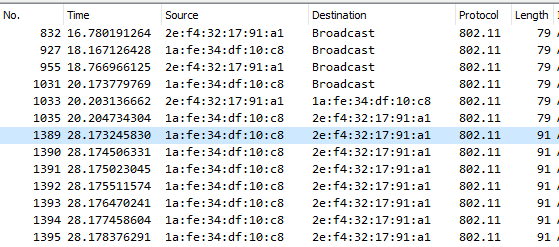
\includegraphics[width=150mm, keepaspectratio]{figures/wireshark_buildup.png}
    \caption{Hálózat felépítése}
    \label{fig:network_buildup}
\end{figure}

A \ref{fig:network_buildup} képen jól látható, hogy kezdetben egyik egység sincs csatlakoztatva, hanem REQUEST\_PARENT típúsú üzeneteket küldenek a broadcast címre. Az 1033-as csomagnál látszik, hogy a 2E-vel kezdőd eszköz lett a route és ő küldi ACCEPT\_CHILD utasítást, majd erre válaszolva érkezik az ACCEPT\_PARENT és a továbbiakban már csak a STATUS üzenet küldése zajlik.

\begin{figure}[th!]
    \centering
    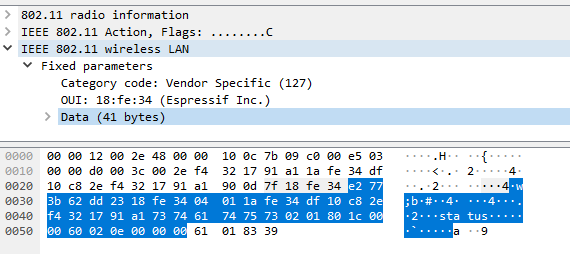
\includegraphics[width=150mm, keepaspectratio]{figures/wireshark_status.png}
    \caption{STATUS üzenet felépítése}
    \label{fig:network_status_format}
\end{figure}

\begin{figure}[!ht]
    \centering
    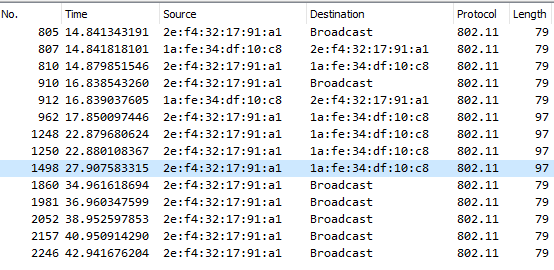
\includegraphics[width=150mm, keepaspectratio]{figures/wireshark_broke.png}
    \caption{Gyökér egység kiesése}
    \label{fig:network_broke}
\end{figure}

A \ref{fig:network_broke} ábrán egy működő hálózat esetén a gyökér egysége kiesése látható. A 962-es üzenetig a hálózat felépítése látszik. Az 1492-es üzenet az utolsó sikeres átküldött STATUS üzenet. Ezután 2E kezdetű egységben lévő időtúlépés számláló értéke, eléri a maximumát és újra visszavált szülő keresési üzemmódban. Mivel nem kap a REQUEST\_PARENT üzeneteire választ, önmagát nevezi ki új gyökér egységnek.

\clearpage

\subsection{Hálózati sávszélesség}
A hálózati sávszélesség méréséhez készítettem egy külön alkalmazást az eszköre, ami még az első és az utolsó átküldött csomag közötti időtartamot. Különböző méretű és mennyiségű csomag esetében az eredmények

\begin{table}[ht]
	\footnotesize
	\centering
	\begin{tabular}{| c | c | c | }
		\toprule
		csomagméret & 10 db & 100 db \\
		\midrule
        10 bájt & 389ms & 3850ms  \\
        \hline
        100 bájt & 398ms & 3712ms  \\
        \hline
		233 bájt & 376ms & 3697ms \\
		\bottomrule
	\end{tabular}
	\caption{ESPNOW üzenetek átviteli ideje}
	\label{tab:esp_now_measurements}
\end{table}

A \ref{tab:esp_now_measurements} táblázat alapján jól látszik, hogy a különböző méretű adatcsomagot úgyanúgy egy üzenetként küldi el és ez nem okoz plusz késleltetési időt. A csomagok számának növelésével pedig arányos növekedik az átküldésükhez szükséges időtartam is.

233 bájt méretű csomagok estében 3697 ms-os késleltetéssel számolva, megkapjuk 50,419 kbit/s sávszélességet.

\[ (233 * 8 * 100) / 3.697 =  50419 \, bit/s \]

\subsection{Fogyasztás}
Az eszköz áramfelvételének mérését az áramkör VIN bementére adott 12 V-os feszültség mellett végeztem el. Az átlagos áram felvétele az eszközönek normál működés esetén \textbf{98.2 mA}. A mikrokontrollert mély alvó állapotba helyezzük, akkor ez a fogyasztás \textbf{17 mA}-ra csökken.